\chapter{Iteración 8}

\begin{quotation}[Leader]{Nelson Mandela (1918--2013)}
It always seems impossible until it’s done.
\end{quotation}

\begin{abstract}
Esta iteración queda reservada para la última fase de desarrollo dentro de la planificación
iterativa de la memoria. Su objetivo es recoger las funcionalidades finales, su diseño, la
implementación realizada y los resultados obtenidos una vez quede cerrada esta entrega.
\end{abstract}

\section{Análisis de características}
En esta iteración se documentarán las funcionalidades seleccionadas del \textit{backlog}
para consolidar la versión final desarrollada durante la fase de ejecución.

\section{Diseño}
Este apartado recogerá las decisiones de diseño adoptadas para las funcionalidades de la
iteración, así como su impacto sobre la arquitectura existente.

\section{Implementación}
Aquí se detallará la implementación realizada, indicando los principales cambios técnicos y
los elementos integrados en el proyecto durante la iteración.

\section{Resultados}
En esta sección se resumirán los resultados obtenidos tras la validación de las
funcionalidades desarrolladas.

\begin{table}[h!]
    \centering
    \begin{coolTable}{lr}{2}
    {Horas de la iteración 8}
    \textbf{Horas reales (Adolfo Borrego González)} & Pendiente de ajustar \\
    \textbf{Horas reales (Germán Sánchez Carmona)} & Pendiente de ajustar \\
    \textbf{Horas reales acumuladas hasta esta iteración} & Pendiente de ajustar \\
    \end{coolTable}
    \caption{Resumen de horas reales de la iteración 8.}
\end{table}

\begin{figure}[htbp]
\begin{center}
\missingfigure{Sustituir por el diagrama UML de resultado de la iteración 8}
% 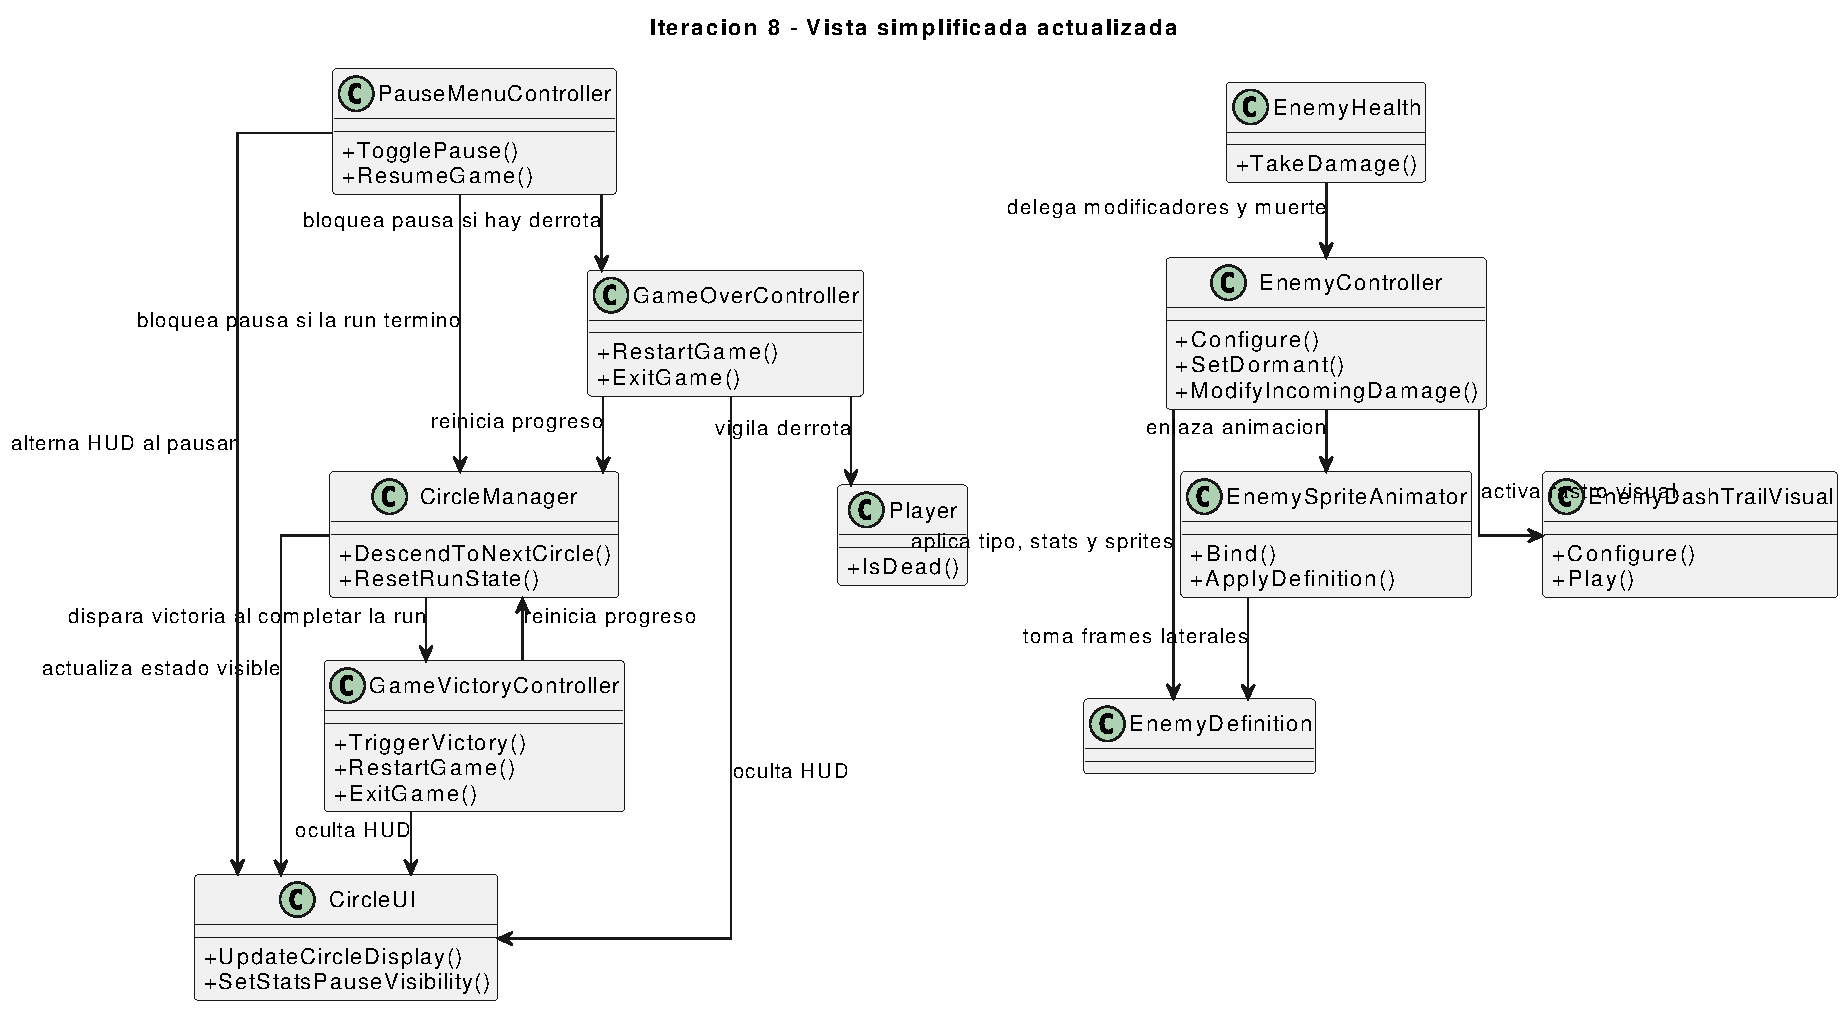
\includegraphics[width=\textwidth]{figures/iteracion8_resultado_uml.pdf}
\caption{Diagrama UML de resultado de la iteración 8}
\label{fig:uml-resultado-iteracion8}
\end{center}
\end{figure}
